\documentclass[12pt,letterpaper,onecolumn,oneside]{article}
\usepackage{graphicx}
\usepackage{float}
\usepackage{multirow}
\usepackage{fixltx2e}
\usepackage{amsmath}
\usepackage{amsfonts}
\usepackage{amsthm}
\usepackage{array}
\usepackage{hyperref}
\usepackage[all]{hypcap}
\usepackage{setspace}
\usepackage{fullpage}

\numberwithin{equation}{section}
\numberwithin{figure}{section}

\newcommand{\ket}[1]{|#1\rangle}

\newtheorem*{Claim}{Claim}

\begin{document}

\title{Stylometry for Online Forums}
\author{Kurt Barry\\
Katherine Luna}
\date{
\begin{center}
CS 229 : Machine Learning\\
Stanford University\\
Autumn Quarter 2012
\end{center}
}

\begin{singlespace}
\maketitle
\end{singlespace}

\section{Introduction}
One of the world wide web's most integral features is the possibility, in principal, of complete anonymity. Though today's web is not anonymous by default, tools like Tor \cite{Tor}, encryption, and 
careful browsing habits can render users difficult to trace and hamper the association of multiple online identities with a single behind-the-scenes individual. While this may be a good thing for political dissidents 
living under oppressive regimes, in other circumstances it would be desirable to remove anonymity to whatever extent possible, e.g.\ in the case of law enforcement monitoring the communications of criminals or 
terrorists over cyber-channels. In particular, the discussion forums of such malicious actors are of great interest. Interesting questions include: who are these people (could anonymous posters in forums be linked to 
Facebook accounts)? On what other sites do they post? Are any of them using multiple usernames (i.e. how many distinct individuals exist in an organization)?

This project applies machine learning techniques to perform stylometric analysis on online forum posts. Stylometry, the study of linguistic style, was used long before the internet existed to resolve historical 
authorship disputes. In the information age, it has been studied as a means to identify bloggers. It is essentially the only tool one has to attempt to reveal or track anonymous entities in web forums. This 
environment presents challenges, however. The very short length of many forum posts yields little stylometric information. Many users are only active on a forum for a brief time, making few posts before their 
activity ceases. It is an open question as to what extent stylometry can succeed in such an environment.

\section{Data}
The data were obtained by scraping posts from an online forum (name omitted to respect privacy) via a custom-written PHP script. The collected corpus contains 331 unique usernames and 16,052 posts. A small core of 
long-term participants accounts for a majority of these posts; the 31 most frequent posters are responsible for 73\% of all posts. The six most frequent posters account for 41\% of all posts. Some basic 
sanitization was performed, primarily removing quotations to prevent confusing text written by different authors.

\section{Methods}
There are essentially two components to stylometry: feature selection and classification algorithm. Most features were selected from previous literature \cite{anonymouth,stanford}, though a few, like 
time-of-posting and use of emoticons, were unique to this project. Information gain was used to select the most useful features. This quantity is defined, for a feature distributed among posts according to a 
probability distribution \(X\), as: \(IG(X) = H(Y) - H(Y|X)\). \(H(Y)\) is the entropy of the probability distribution for a post to be written by each author; \(H(Y|X)\) is the conditional entropy of the author 
distribution given the distribution of the feature in question. Since all the features were continously-valued, they had to be discretized before information gain could be calculated. This was done via a heuristic 
algorithm based on the notion that bins should on average have a width proportional to the average standard deviation of that feature among all users, but should also contain roughly equal numbers of examples. We 
used the top fifteen features as ranked by information gain. Using more features than this number involved diminishing returns, likey linked in part to high frequency of short, ambiguously authored posts. In some 
cases adding features even worsened performance. Keeping the list short has the added benefit of computational efficiency.

The top features can be seen in Figure \ref{infogain}. Interestingly, the same set of features was found to be best for all users with \(>\) 50 posts and \(>\) 500 posts, though the ordering changed slightly. It is 
interesting that some useful features are either not available or less useful in other stylometric applications. For example, time-of-posting makes little sense in the context of books or newspaper articles 
(although it could conceivably be useful in the blogosphere). Others, like the fraction of characters that are punctuation, the average number of apostrophes per word, and the fraction of characters that are upper case, 
are likely so useful in forums precisely because there is little incentive for individuals to follow the established rules of English orthography beyond making themselves understandable. This is an important aspect of 
forum stylometry that differs from other applications.

\begin{figure}[H]
 \centering
  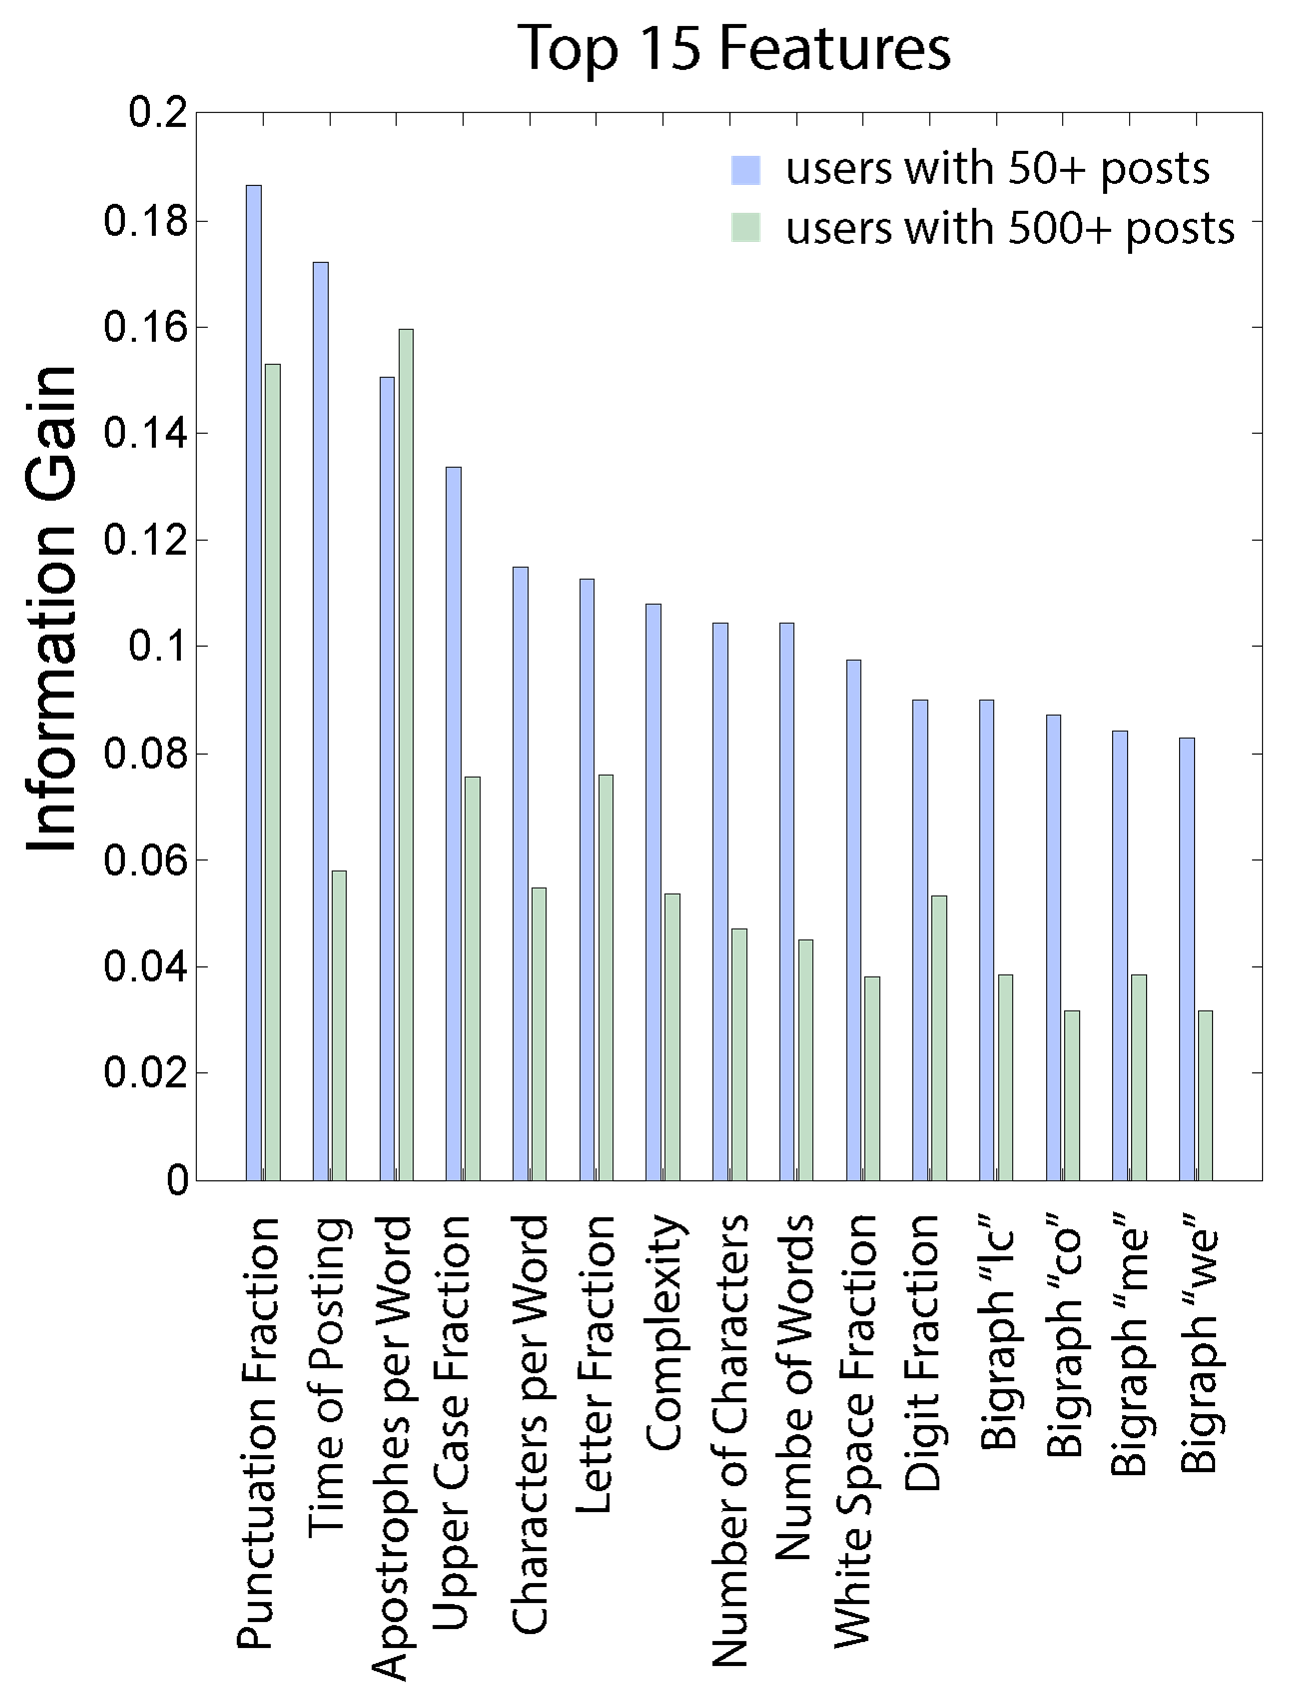
\includegraphics[scale=0.4]{TopFeatures.png}
  \caption{\textbf{\footnotesize{The top features, ranked by information gain.}}}
  \label{infogain}
\end{figure}

Two algorithms were used. The first was a multinomial Naive Bayes classifier. It was implemented in Python and used the same discretizations used to calculate the information gain. The second was a support vector 
machine (SVM). Rather than implement our own, we used the SVC support vector machine in the open source \verb+scikit-learn+ \cite{scikit-learn} Python module (which itself uses libsvm \cite{libsvm}). 
Multi-class classification is handled by constructing a binary classifier for each pair of users; the decision process is then treated as an ``election'' in which each classifier ``votes'' for a particular user 
\cite{libsvm}. Since the various features all had different ranges, we rescaled the extracted values to have mean 0 and standard deviation 1 before running the SVM. A number of different kernels were experimented 
with: linear, exponential (\(e^{-\gamma <x,x'>^2}\)), and polynomial kernels of various degree. The best performing kernel was found to be quadratic in the inner product of the feature vectors, specifically 
\(K(x,x') = (0.5<x,x'>+9)^2\). To give some quantitative sense of this kernel's superiority, its accuracy is roughly six percentage points better than a linear kernel. Using higher-degree polynomials does not yield 
improvements in accuracy.

\section{Results}
The performance of these algorithms is summarized in Table \ref{numbers}. Two (non-disjoint) subsets of users were tested: those with more than 500 posts (six individuals) and those with more than 50 posts 
(forty-six individuals). Ten-fold cross validation was used to assess the accuracies. The selected folds were the same for both algorithms. In all cases random chance is outperformed by a significant amount. 
Though the accuracy is reduced for the larger set of users, it is actually better compared to random than for fewer users. A major factor limiting performance is very short posts, which contain little stylistic 
information and are thus difficult to attribute. As an example of this, training and testing on only posts with more than ten words for those users with greater than 500 posts improves the accuracies to 
44.6 and 57.1 percent, for Naive Bayes and the SVM, respectively. To give some indication of the challenges involved in separating the data with the chosen features, Figure \ref{SVM_pic} shows an example SVM 
classification using three posters and two features. The substantial overlap of the data highlights the need to use many features and nonlinear decision boundaries.

\begin{table}
\begin{center}
  \begin{tabular}{| c | c | c | c |}
    \hline
      & \multicolumn{3}{|c|}{Algorithm Accuracy} \\
    \hline
     & Naive Bayes & SVM & Random Chance \\ \hline
    users with \(>\) 500 posts & 40.5\% & 53.8\% & 16.7\% \\ \hline
    users with \(>\) 50 posts & 20.4\% & 32.9\% & 2.2\% \\ \hline
  \end{tabular}
  \caption{\textbf{\footnotesize{Algorithm performance on the top six and top forty-six most frequent posters, compared to random chance.}}}
  \label{numbers}
\end{center}
\end{table}

\begin{figure}[H]
 \centering
  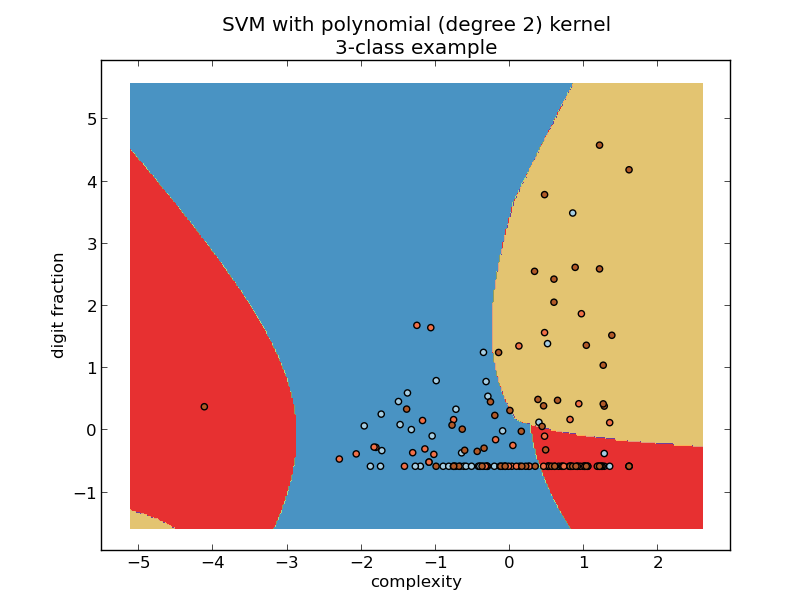
\includegraphics[scale=0.4]{SVMpic.png}
  \caption{\textbf{\footnotesize{An example SVM classification with limited data, using only two features.}}}
  \label{SVM_pic}
\end{figure}

\section{Conclusions}
This project represents proof-of-concept for stylometry in online forums where data is often noisy and less abundant than in other written environments. Certainly improvements can be made. It is difficult to 
imagine significant progress on attributing extremely short posts (e.g., ``Welcome to the forum!''), but the use of more extensive feature sets may improve accuracy for longer posts. Examples of promising features 
include ``function word'' frequencies (see \cite{stanford}) and recognition of particular phrases or grammatical constructs preferred by posters (which would require some level of natural language processing to 
extract). 

\begin{thebibliography}{1}
\begin{singlespace}

  \bibitem{Tor}
Tor Project: Anonymity Online \url{https://www.torproject.org/}

  \bibitem{anonymouth}
Andrew W.E. McDonald, Sadia Afroz, Aylin Caliskan, Ariel Stolerman, Rachel Greenstadt ``Use Fewer Instances of the Letter ``i'': Toward Writing Style Anonymization'' The 12th Privacy Enhancing Technologies Symposium. 2012.

  \bibitem{stanford}
Arvind Narayanan, Hristo Paskov, Neil Zhenqiang Gong, John Bethencourt, Emil Stefanov, Eui Chul Richard Shin, Dawn Song: On the Feasibility of Internet-Scale Author Identification. IEEE Symposium on Security and Privacy 2012: 300-314

  \bibitem{scikit-learn}
Pedregosa et al., Scikit-learn: Machine Learning in Python, JMLR 12, pp. 2825-2830, 2011.

  \bibitem{libsvm}
Chih-Chung Chang and Chih-Jen Lin, LIBSVM : a library for support vector machines. ACM Transactions on Intelligent Systems and Technology, 2:27:1--27:27, 2011. Software available at \url{http://www.csie.ntu.edu.tw/~cjlin/libsvm}

\end{singlespace}
\end{thebibliography}

\end{document}
